\documentclass[tikz,border=10pt]{standalone}
\begin{document}
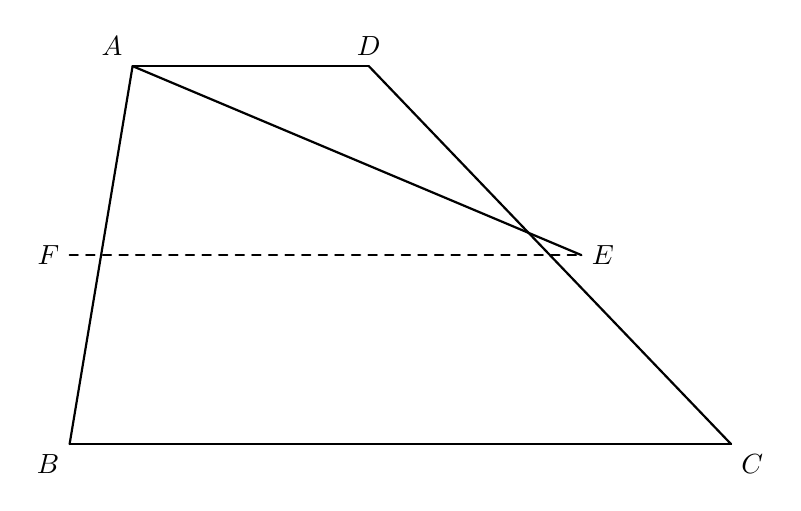
\begin{tikzpicture}[line cap=round,line join=round,thick]

\coordinate (A) at (1.2,4.8);
\coordinate (B) at (0.4,0.0);
\coordinate (C) at (8.8,0.0);
\coordinate (D) at (4.2,4.8);
\coordinate (E) at (6.9,2.4);
\coordinate (F) at (0.4,2.4);

\draw (A) -- (B);
\draw (B) -- (C);
\draw (A) -- (D);
\draw (D) -- (C);
\draw (A) -- (E);
\draw[dashed] (F) -- (E);

\node[above left] at (A) {$A$};
\node[below left] at (B) {$B$};
\node[below right] at (C) {$C$};
\node[above] at (D) {$D$};
\node[right] at (E) {$E$};
\node[left] at (F) {$F$};

\end{tikzpicture}
\end{document}
